% !TEX program = xelatex
\documentclass[a4paper,singleside,12pt]{report}
% \documentclass[a4paper,twoside,12pt]{report} % For printed double-sided version

% University of Bologna thesis style.
% Compile with XeLaTeX because ai_bo_thesis uses fontspec.
\usepackage{ai_bo_thesis}

\usepackage[english]{babel}

% Main font
\setmainfont{Times New Roman}

% Mathematics and symbols
\usepackage{amsmath}
\usepackage{amssymb}
\usepackage{mathtools}

% Tables
\usepackage{booktabs}
\usepackage{array}
\usepackage{multirow}
\usepackage{longtable}

% Figures
\usepackage{graphicx}
\usepackage{float}
\usepackage{subcaption}
\usepackage{tikz}
\usetikzlibrary{positioning, arrows.meta, decorations.pathreplacing, calc}
% Units and numbers
\usepackage{siunitx}

% Text and URLs
\usepackage{xurl}
\usepackage{csquotes}

% Algorithms / pseudocode, if needed later
% \usepackage{algorithm}
% \usepackage{algpseudocode}

% Bibliography
\usepackage[
    backend=biber,
    style=trad-plain,
    sorting=none,
    giveninits=true
]{biblatex}
\addbibresource{bibliography/references.bib}

% Figure path
\graphicspath{{figures/}}

% Hyperref should usually be loaded near the end of the preamble
\usepackage[hidelinks]{hyperref}

% Clever references after hyperref, optional but useful
\usepackage[nameinlink,noabbrev]{cleveref}

\begin{document}

    % ----------------------------------------------------------------------
    % Frontispiece metadata
    % ----------------------------------------------------------------------

    \title{Graph-Theoretic Analysis of Scalp EEG Functional Connectivity for Epileptic Seizure Prediction}

    \topic{Cognition and Neuroscience}

    \candidate{Leila Sadakbayeva}

    % Confirm final supervisor / co-supervisor roles before submission.
    \supervisor{Prof.~Francesca Starita}
    \cosupervisor{& Prof.~Saverio Giallorenzo}

    \academicyear{2025-2026}

    % Update according to the official graduation session.
    \session{ to be confirmed}

    \frontispiece

    % ----------------------------------------------------------------------
    % Abstract
    % ----------------------------------------------------------------------

    \chapter*{Abstract}

    Epileptic seizure prediction is a challenging problem in biomedical signal
    processing, with potential relevance for clinical monitoring and patient
    safety. This thesis investigates whether pre-ictal changes in brain network
    topology can be detected from scalp electroencephalography (EEG) recordings
    using functional connectivity and graph-theoretic analysis.

    The proposed pipeline is evaluated on the CHB-MIT scalp EEG dataset. EEG
    recordings are segmented into baseline and pre-ictal windows preceding
    seizure onset. For each segment, functional connectivity matrices are
    computed across multiple frequency bands using coherence, weighted Phase Lag
    Index, and amplitude envelope correlation. These matrices are interpreted as
    weighted brain networks from which graph metrics such as clustering
    coefficient, global efficiency, characteristic path length, small-worldness,
    modularity, betweenness centrality, and assortativity are extracted.

    An initial exploratory analysis on subject chb01 shows that delta-band wPLI
    mean betweenness centrality decreases consistently before seizures and
    survives false discovery rate correction in a repeated-measures ANOVA. Since
    this result is obtained from a single-subject pilot analysis, it is treated
    as preliminary and used to guide further validation on additional subjects
    and exploratory prediction experiments.

    \cleardoublepage

    % ----------------------------------------------------------------------
    % Tables of contents
    % ----------------------------------------------------------------------

    \toc
    \figstoc
    \tablestoc

    \begintext

    % ----------------------------------------------------------------------
    % Main chapters
    % ----------------------------------------------------------------------

    % \chapter{Introduction}

Epilepsy is a neurological disorder characterized by recurrent seizures. The ability to identify preictal changes in electroencephalography (EEG) could support seizure forecasting and improve patient safety.

This chapter will introduce the research problem, motivation, thesis objectives, and overall structure of the work.

% Figure placeholder:
% \begin{figure}[htbp]
%     \centering
%     \includegraphics[width=0.8\textwidth]{figures/example_figure.png}
%     \caption{Example figure caption.}
%     \label{fig:example}
% \end{figure}



    % \chapter{Background and State of the Art}

This chapter will summarize the clinical and technical background needed for the thesis, including epilepsy, EEG analysis, seizure prediction, functional connectivity, and graph theory.

Prior studies have investigated changes in network organization before seizures. This section will compare relevant methods and position the thesis contribution.

% Table placeholder:
% \begin{table}[htbp]
%     \centering
%     \caption{Example literature comparison table.}
%     \label{tab:literature}
%     \begin{tabular}{lll}
%         \toprule
%         Study & Dataset & Method \\
%         \midrule
%         Placeholder & Placeholder & Placeholder \\
%         \bottomrule
%     \end{tabular}
% \end{table}



    \chapter{Dataset and Preprocessing}
\label{chap:dataset-preprocessing}

The goal of this stage is to transform raw scalp EEG recordings into a structured
set of seizure-centred windows suitable for functional connectivity estimation
and graph-theoretic analysis. The pipeline is designed to be reproducible and
modular: the dataset is first screened according to explicit eligibility
criteria, raw EEG recordings are then preprocessed, standardized temporal
windows are extracted around seizure onset, and each window is divided into
short epochs. The resulting arrays are used as input for the connectivity
computation described in \cref{chap:connectivity-graph-features}.

\section{CHB-MIT Dataset}
\label{sec:chbmit-dataset}

The experimental work presented in this thesis is based on the CHB-MIT Scalp
EEG Database, a publicly available dataset distributed through PhysioNet and
widely used in seizure detection and seizure prediction research
\cite{PhysioNet-chbmit-1.0.0}. The dataset contains long-term scalp EEG
recordings acquired from pediatric patients with intractable epilepsy during
clinical monitoring. The recordings provide a valuable resource for studying
the temporal evolution of brain activity before and during epileptic seizures.

A note on terminology is necessary because the CHB-MIT dataset distinguishes
between subjects and cases. According to the official PhysioNet description,
the database consists of \num{23} cases obtained from \num{22} pediatric
subjects, since case \texttt{chb21} corresponds to a later recording session of
the same individual as \texttt{chb01}. However, the downloadable dataset used
in this thesis contains case folders ranging from \texttt{chb01} to
\texttt{chb24}. The additional case \texttt{chb24} was added after the original
release and is not included in the \texttt{SUBJECT-INFO} metadata file. For
consistency, the terms \emph{subject}, \emph{case}, and \emph{subject ID} are
used throughout the remainder of this thesis to refer to the CHB-MIT dataset
identifiers rather than necessarily to unique biological individuals.

The EEG recordings are stored in European Data Format (EDF) files, while
seizure onset and offset times are provided through accompanying annotation
files and metadata. These annotations enable a seizure-centred analysis, since
they allow temporal windows to be defined relative to seizure onset and make it
possible to investigate changes in brain dynamics during the preictal period.

The present work adopts a sensor-level approach to functional brain network
analysis. Each bipolar EEG channel is treated as a node in a functional
network, whereas pairwise functional connectivity estimates define weighted
edges between nodes. This approach avoids the need for source reconstruction,
which would require subject-specific anatomical information that is not
available in the CHB-MIT dataset. At the same time, it imposes an important
methodological requirement: network nodes must remain comparable across
subjects, seizures, frequency bands, connectivity measures, and temporal
windows.

To ensure such comparability, a fixed montage consisting of \num{22} bipolar
EEG channels was used throughout the analysis. Maintaining a consistent set of
network nodes is essential for meaningful comparisons of connectivity matrices
and graph-theoretical metrics across recordings. Consequently, only recordings
containing the complete required montage were considered eligible for further
analysis.

\section{Dataset Screening and Eligibility Criteria}
\label{sec:dataset-screening-eligibility}

Not all annotated seizures in the original dataset satisfied the requirements
of the present study. Therefore, a dedicated screening procedure was performed
before preprocessing in order to identify recordings that provided both the
necessary temporal context and the complete channel configuration.

A seizure was retained only if it satisfied two eligibility requirements. First,
at least \SI{540}{\second} of EEG data had to be available before seizure onset.
This corresponds to the \SI{9}{\minute} preictal interval used to extract three
consecutive \SI{3}{\minute} windows before the seizure. Second, the recording
had to contain the complete fixed \num{22}-channel bipolar montage used in this
thesis. Since each channel is later treated as a graph node, missing channels
would produce graphs with different node sets and would make graph metrics
incomparable across seizures.

The overall screening procedure is summarized in
\cref{fig:dataset-screening-flowchart}. The exclusion categories are not
mutually exclusive: some seizures failed both the temporal and channel
requirements.

\begin{figure}[H]
    \centering
    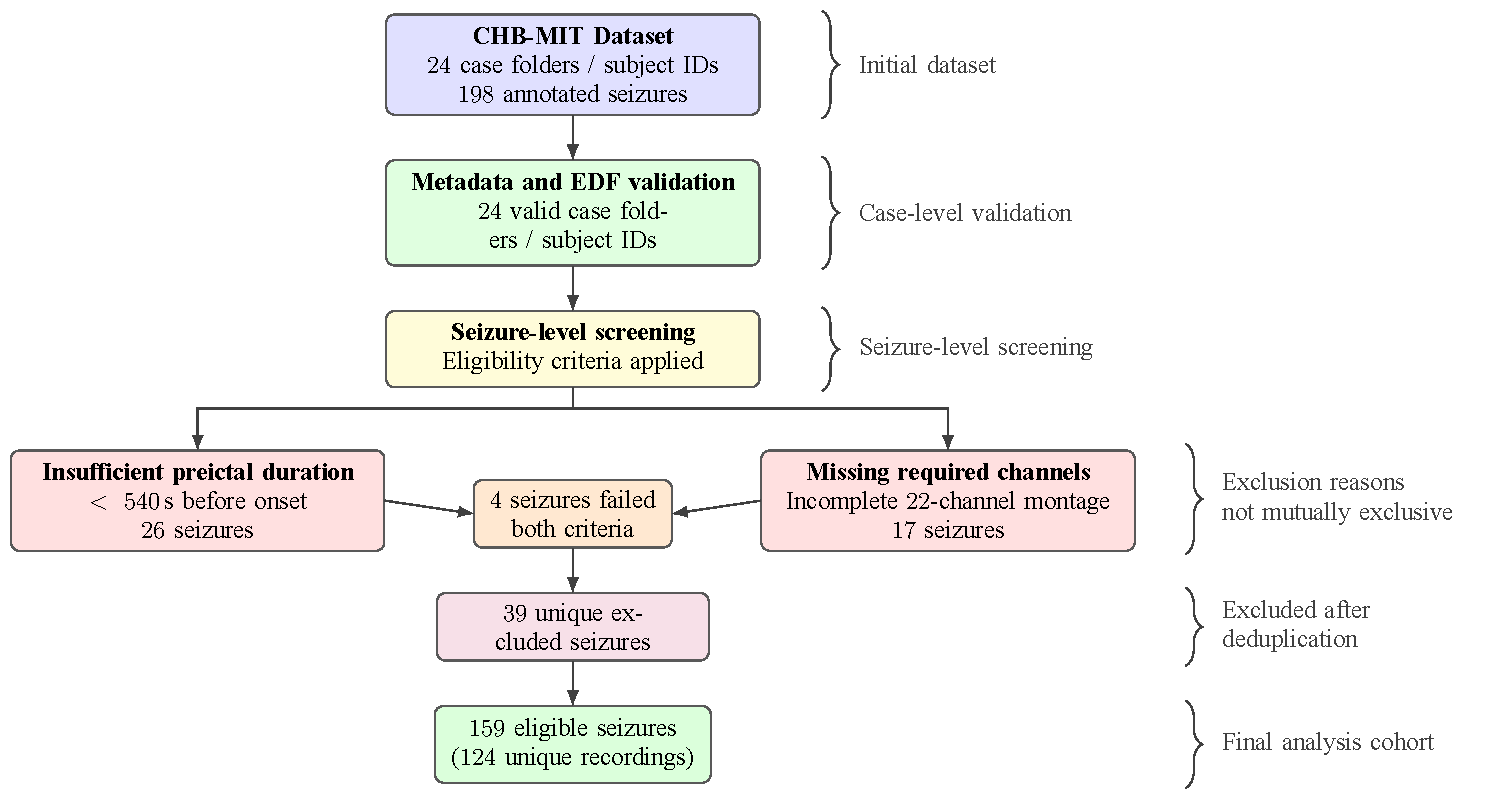
\includegraphics[width=0.95\textwidth]{figures/flowchart.pdf}
    \caption{Flowchart of the dataset screening procedure and seizure eligibility criteria.}
    \label{fig:dataset-screening-flowchart}
\end{figure}

The final screening outcome is reported in
\cref{tab:dataset-screening-summary}. In total, \num{198} annotated seizures
were screened. Of these, \num{159} seizures were retained and \num{39} were
excluded. The retained seizures corresponded to \num{124} unique EEG recordings,
and every screened case folder / subject ID contributed at least one usable
seizure.

\begin{table}[H]
    \centering
    \begin{tabular}{lr}
        \toprule
        Screening quantity & Count \\
        \midrule
        Case folders / subject IDs screened & 24 \\
        Case folders / subject IDs with seizure annotations & 24 \\
        Case folders / subject IDs with readable metadata & 24 \\
        Case folders / subject IDs with at least one usable seizure & 24 \\
        Annotated seizures screened & 198 \\
        Usable seizures retained & 159 \\
        Excluded seizures & 39 \\
        Unique usable recordings & 124 \\
        \bottomrule
    \end{tabular}
    \caption{Summary of dataset screening and seizure eligibility.}
    \label{tab:dataset-screening-summary}
\end{table}

Among the excluded seizures, \num{26} had less than \SI{540}{\second} of
available preictal data and \num{17} were missing one or more channels from the
required bipolar montage. Since \num{4} seizures failed both criteria, the sum
of the individual exclusion reasons is greater than the number of unique
excluded seizures.

The distribution of usable and excluded seizures across case folders is shown
in \cref{fig:subject-vs-seizures-screening}. The figure shows that the dataset
is not balanced across case folders: some contain only a few annotated seizures,
whereas others contain substantially more. This imbalance is important for the
later statistical analysis, because seizures from the same case folder are not
fully independent observations.

\begin{figure}[H]
    \centering
    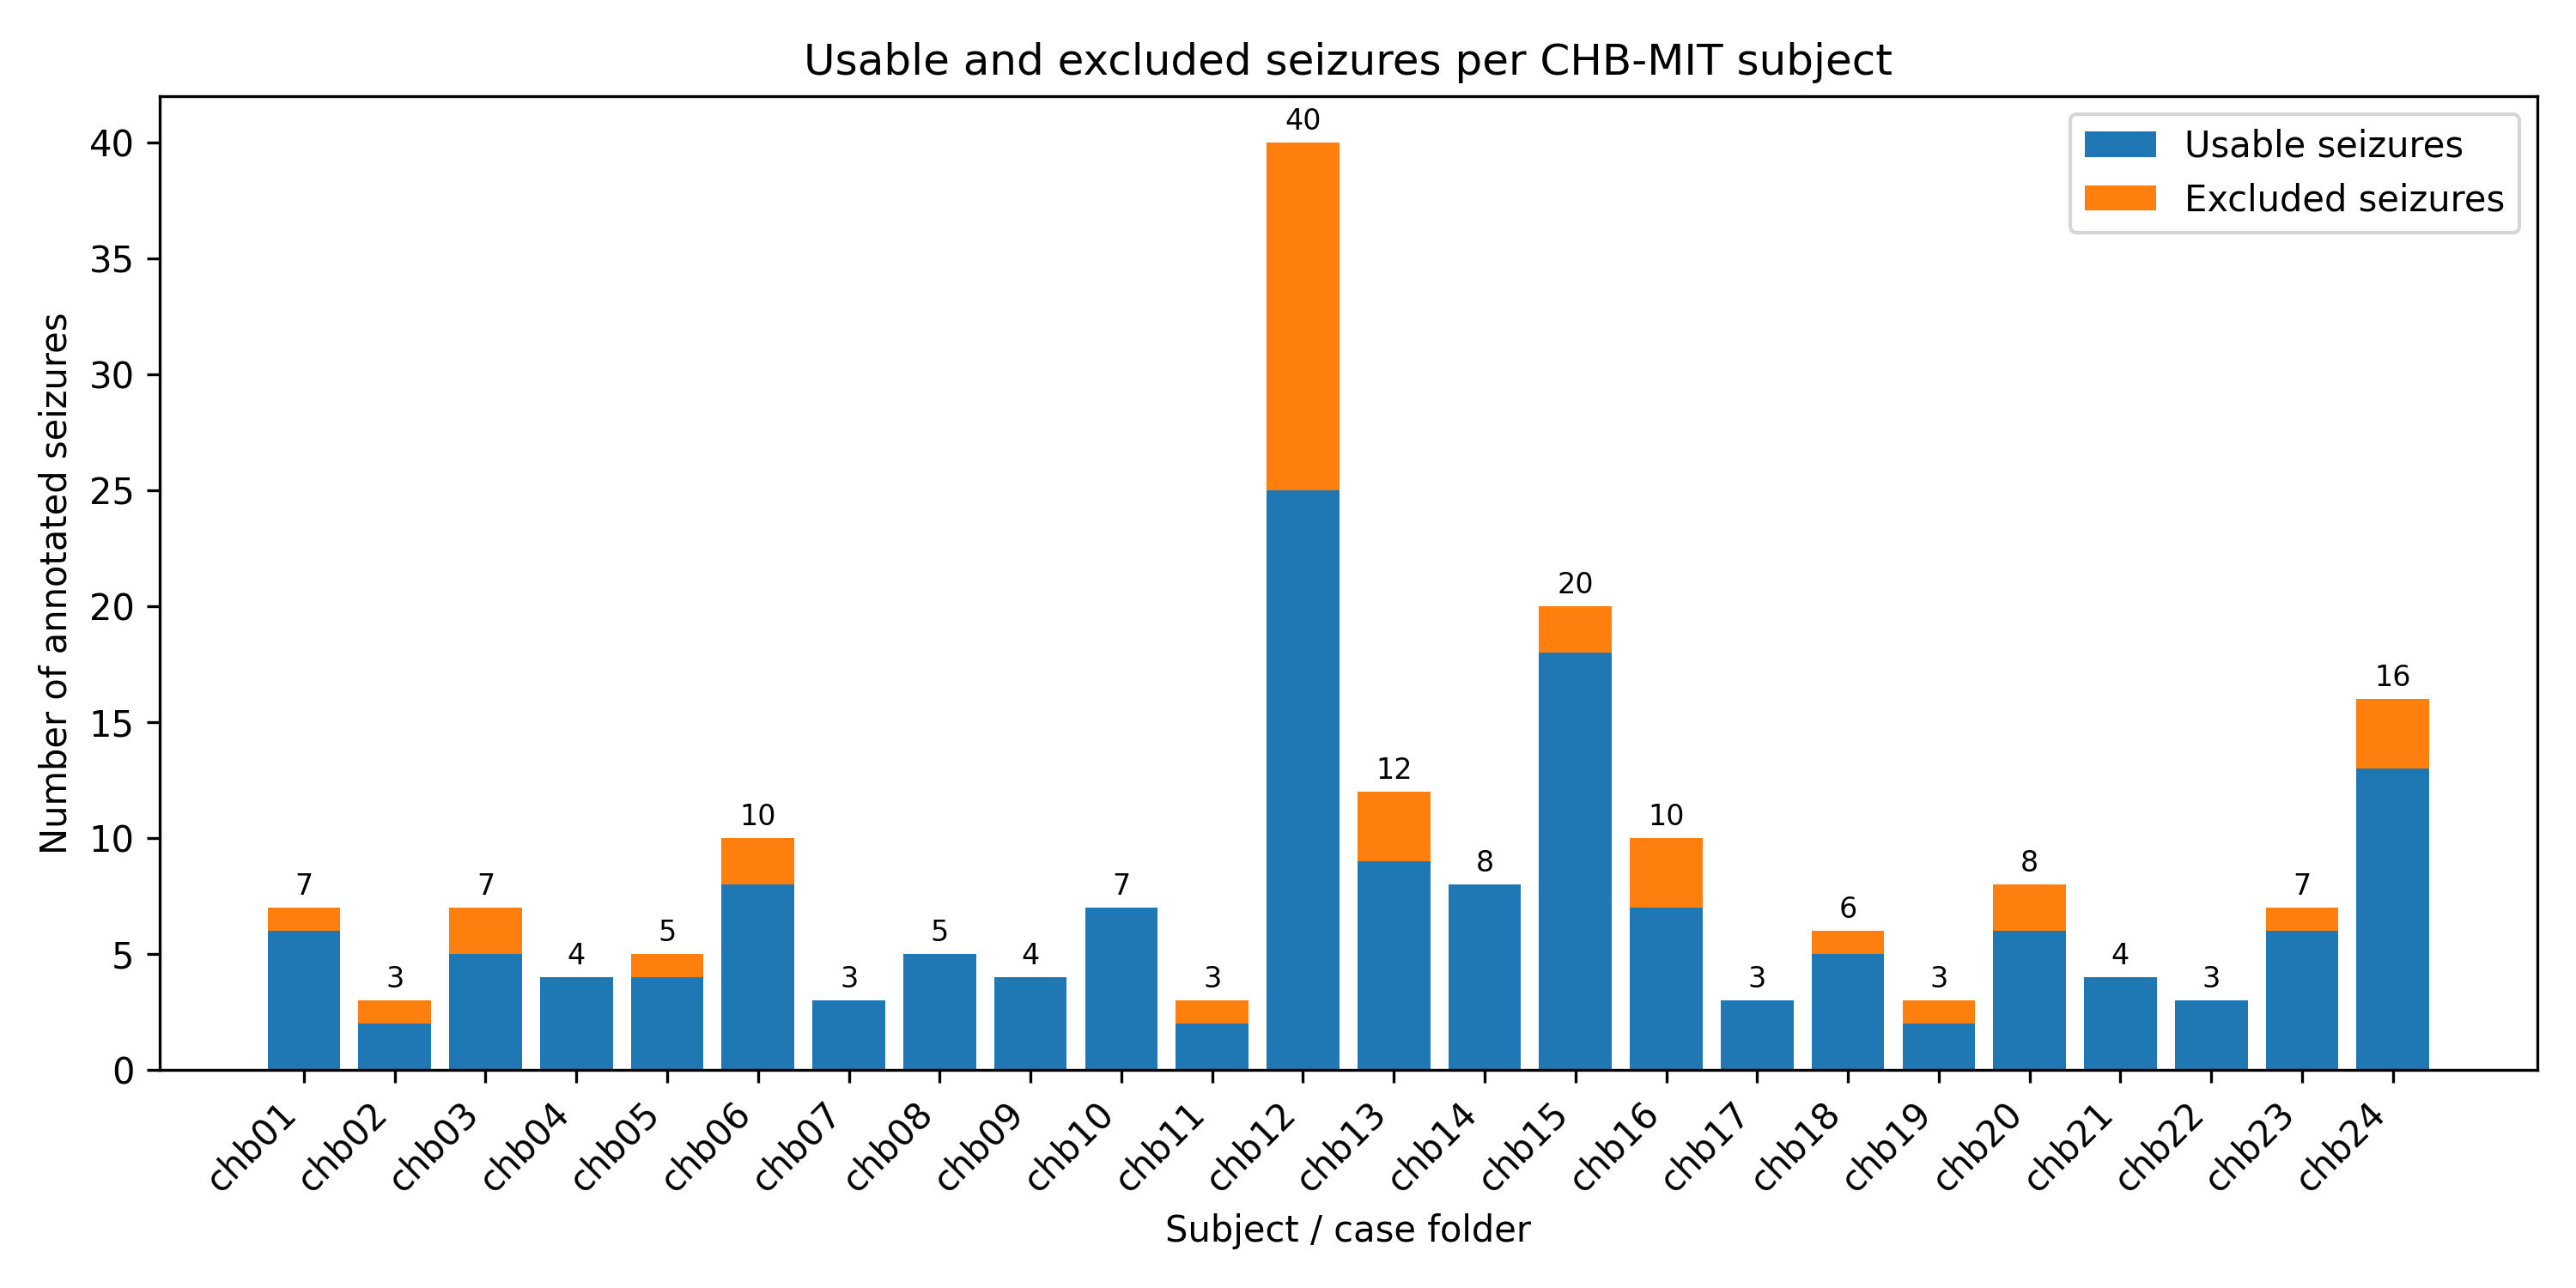
\includegraphics[width=\textwidth]{figures/subject_vs_seizures_screening.png}
    \caption{Number of usable and excluded annotated seizures for each CHB-MIT
    case folder / subject ID after dataset screening. The number above each bar
    indicates the total number of annotated seizures for that case.}
    \label{fig:subject-vs-seizures-screening}
\end{figure}

\section{EEG Preprocessing}
\label{sec:eeg-preprocessing}

After dataset screening, all usable seizure-linked recordings were passed to a
standardized preprocessing pipeline. The purpose of this stage was to transform
the raw EDF recordings into a consistent set of EEG recordings with the same
sampling frequency, channel set, channel order, and filtering characteristics.
This was necessary because the subsequent connectivity and graph-theoretical
analysis requires comparable network nodes across all subjects, seizures, and
time windows.

\subsection{Selection of Recordings for Preprocessing}
\label{subsec:preprocessing-recording-selection}

The preprocessing pipeline used the seizure eligibility table produced during
dataset screening as its input. Only recordings associated with at least one
usable seizure were selected. If multiple usable seizures occurred in the same
EDF recording, the recording was processed only once and reused during the later
segmentation stage. This avoided redundant preprocessing while preserving the
link between each seizure, subject/case folder, and original recording file.

Each selected EDF file was loaded into memory using MNE-Python. The absolute
measurement date stored in the EDF metadata was removed before saving the
processed file, because some CHB-MIT headers contain dates that are outside the
range accepted by the FIF file format. This operation does not affect the
analysis, since all seizure annotations and window definitions in this thesis
are expressed in seconds relative to the beginning of each recording rather than
in absolute calendar time.

\subsection{Channel Selection and Montage Standardization}
\label{subsec:channel-selection-montage-standardization}

A fixed set of \num{22} bipolar EEG channels was retained for all recordings.
These channels define the graph nodes used in the functional connectivity
analysis. The required montage was:

\begin{center}
\begin{tabular}{llll}
\toprule
\texttt{FP1-F7} & \texttt{F7-T7} & \texttt{T7-P7} & \texttt{P7-O1} \\
\texttt{FP1-F3} & \texttt{F3-C3} & \texttt{C3-P3} & \texttt{P3-O1} \\
\texttt{FP2-F4} & \texttt{F4-C4} & \texttt{C4-P4} & \texttt{P4-O2} \\
\texttt{FP2-F8} & \texttt{F8-T8} & \texttt{T8-P8} & \texttt{P8-O2} \\
\texttt{FZ-CZ} & \texttt{CZ-PZ} & \texttt{P7-T7} & \texttt{T7-FT9} \\
\texttt{FT9-FT10} & \texttt{FT10-T8} & & \\
\bottomrule
\end{tabular}
\end{center}

After loading each recording, channel names were normalized to a canonical
format and the recording was checked for the presence of all required channels.
Recordings missing one or more channels from the required bipolar montage were
excluded during dataset screening. Consequently, all recordings retained for
preprocessing contained the complete \num{22}-channel montage.

After validation, the channels were explicitly reordered according to the fixed
montage. This ensured that the same channel index corresponded to the same
bipolar derivation in every preprocessed recording and in every later
connectivity matrix.

\subsection{Handling of Duplicate \texorpdfstring{\texttt{T8-P8}}{T8-P8} Channels}
\label{subsec:t8-p8-duplicate-handling}

Some CHB-MIT recordings contain duplicated versions of the \texttt{T8-P8}
channel. When loaded by MNE-Python, these duplicated channels may appear with
suffixes such as \texttt{T8-P8-0} and \texttt{T8-P8-1}. To preserve a single
canonical version of this bipolar channel, the duplicate channel
\texttt{T8-P8-1} was removed. The retained channel \texttt{T8-P8-0} was then
renamed to the canonical label \texttt{T8-P8}.

This procedure allowed recordings with this naming convention to be retained
while still enforcing the same \num{22}-channel montage across the full
analysis. Importantly, the duplicate channel was handled before the final
channel check and reordering step, so that the output always contained exactly
one \texttt{T8-P8} channel.

\subsection{Sampling Frequency Verification}
\label{subsec:sampling-frequency-verification}

All retained recordings were verified to have a sampling frequency of
\SI{256}{\hertz}. No resampling was applied. Recordings with a mismatched
sampling frequency would have been rejected during preprocessing, but no such
mismatch was observed among the retained usable recordings.

\subsection{Filtering}
\label{subsec:eeg-filtering}
The EEG signals were filtered at the recording level before segmentation. A
finite impulse response (FIR) band-pass filter was applied between
\SI{0.5}{\hertz} and \SI{47}{\hertz}. The lower cutoff was used to attenuate
slow drifts and very low-frequency baseline fluctuations, consistent with
previous quantitative EEG preprocessing approaches in epilepsy research
\cite{Lanzone2022}. The upper cutoff was chosen to match the frequency range
required for the present connectivity analysis and is consistent with the
\SI{47}{\hertz} upper cutoff used by Vecchio et al. in a pre-seizure
graph-theoretical EEG connectivity study \cite{Vecchio2016}.

The highest frequency band analyzed later in the pipeline was the beta2 band
(\SIrange{20}{30}{\hertz}). Therefore, the \SI{47}{\hertz} upper cutoff retained
the full frequency content required for all analyzed bands while suppressing
higher-frequency activity outside the scope of this study. Since the upper
cutoff frequency was below the \SI{60}{\hertz} power-line frequency, no
additional \SI{60}{\hertz} notch filter was applied in the final preprocessing
pipeline.

Filtering was performed on the continuous recording before seizure-centred
windows were extracted. This avoids applying filters separately to short
segments and reduces the risk of introducing window-specific filtering
artifacts.

\subsection{Artifact Handling}
\label{subsec:artifact-handling}

No additional manual or automatic artifact rejection was performed during this
preprocessing stage. This choice was made to keep the preprocessing procedure deterministic and
reproducible across the full dataset. However, it also means that residual
artifacts may still be present in some retained recordings. This limitation is
considered when interpreting the connectivity and graph-theoretical results.

\subsection{Saving Preprocessed Recordings}
\label{subsec:saving-preprocessed-recordings}

After channel standardization, sampling-frequency verification, and filtering,
each preprocessed recording was saved as an intermediate MNE FIF file
and reused during the segmentation stage. Saving these intermediate files
allowed preprocessing to be separated from later analysis steps and ensured that
all subsequent stages used the same standardized recordings.

A preprocessing log was generated to record the processing status of each
selected recording, including the subject/case identifier, recording file,
sampling frequency, number of retained channels, and any error messages.

\section{Temporal Window Definition}
\label{sec:temporal-window-definition}

After preprocessing, seizure-centred temporal windows were extracted from each
eligible seizure recording. The aim of this step was to describe how functional
connectivity and graph-theoretical properties evolve during the minutes
preceding seizure onset. For this reason, the analysis was organized around one
baseline window and three consecutive preictal windows.

The temporal structure was inspired by the design used by Vecchio et al.,
who investigated graph-theoretical changes during the \SI{9}{\minute} period
preceding seizure onset by dividing this interval into three consecutive
\SI{3}{\minute} windows \cite{Vecchio2016}. The present study adopted the same
preictal window structure, but applied it to a larger scalp EEG dataset and to
multiple connectivity measures and graph metrics.

For each seizure, four windows were defined:

\begin{itemize}
    \item \textbf{Baseline}: a \SI{3}{\minute} interictal window selected from
    the same recording, at least \SI{600}{\second} away from any annotated
    seizure activity;
    \item \textbf{T0}: the interval from \SIrange{9}{6}{\minute} before seizure
    onset;
    \item \textbf{T1}: the interval from \SIrange{6}{3}{\minute} before seizure
    onset;
    \item \textbf{T2}: the interval from \SIrange{3}{0}{\minute} before seizure
    onset.
\end{itemize}

The baseline window was used as a reference period representing interictal EEG
activity within the same recording. To reduce contamination by seizure-related
activity, baseline segments were required to be at least \SI{600}{\second}
away from all annotated seizures in that recording. The baseline selection
therefore used all known seizure intervals in the recording, including seizures
that were not retained for the final analysis, because these intervals still
represent ictal periods.

The three preictal windows T0, T1, and T2 covered the final \SI{9}{\minute}
before seizure onset. This organization allowed the analysis to compare
baseline activity with progressively later preictal periods and to examine
whether network properties changed as seizure onset approached. The use of
fixed-duration windows also ensured that connectivity estimates were computed
from equal amounts of data across all seizures and conditions.

Each window had a duration of \SI{180}{\second}. After extraction, each window
was divided into non-overlapping \SI{2}{\second} epochs. Since the sampling
frequency was \SI{256}{\hertz}, each epoch contained \num{512} samples. Thus,
each saved window had the shape

\[
    90 \times 22 \times 512,
\]

corresponding to \num{90} epochs, \num{22} EEG channels, and \num{512} samples
per epoch. These epoch-level representations were then used for the computation
of frequency-specific functional connectivity matrices.

\section{Frequency Band Decomposition}
\label{sec:frequency-band-decomposition}

Functional connectivity was computed separately within predefined EEG frequency
bands. This was done because epileptic brain dynamics may affect different
frequency ranges in different ways, and graph-theoretical properties can depend
on the spectral content used to define the functional network.

The frequency bands used in this thesis followed the band structure adopted by
Vecchio et al. \cite{Vecchio2016}. In particular, the alpha and beta ranges were
subdivided into narrower bands, allowing potential differences between lower and
higher alpha or beta activity to be examined separately. The analyzed frequency
bands were:

\begin{table}[H]
    \centering
    \begin{tabular}{ll}
        \toprule
        Frequency band & Frequency range \\
        \midrule
        Delta & \SIrange{2}{4}{\hertz} \\
        Theta & \SIrange{4}{8}{\hertz} \\
        Alpha1 & \SIrange{8}{10}{\hertz} \\
        Alpha2 & \SIrange{10}{13}{\hertz} \\
        Beta1 & \SIrange{13}{20}{\hertz} \\
        Beta2 & \SIrange{20}{30}{\hertz} \\
        \bottomrule
    \end{tabular}
    \caption{Frequency bands used for functional connectivity analysis.}
    \label{tab:frequency-bands}
\end{table}

Although gamma-band activity is often considered in EEG studies, it was not
included in the present analysis. The frequency decomposition was predefined to
match the study that motivated the temporal and spectral structure of this
work, which focused on delta, theta, alpha, and beta sub-bands. In addition,
gamma-band scalp EEG is more vulnerable to contamination by muscle activity and
other high-frequency artifacts. Since no dedicated artifact rejection procedure
was applied in this pipeline, the analysis was restricted to frequencies up to
the beta2 band, ending at \SI{30}{\hertz}.

This restriction also kept the number of frequency bands and statistical tests
manageable. Gamma-band connectivity is therefore left as a possible extension
for future work rather than being included in the main analysis.

    \chapter{Connectivity and Graph Features}
\label{chap:connectivity-graph-features}

\section{Overview of Network Construction}
\label{sec:functional-network-construction-overview}

After preprocessing and temporal segmentation, each seizure-related EEG window
was represented as a three-dimensional array containing \num{90}
non-overlapping epochs, \num{22} bipolar EEG channels, and \num{512} samples per
epoch. These segmented EEG windows formed the input to the functional
connectivity pipeline. The purpose of this stage was to transform each
time-windowed EEG segment into a set of functional brain networks that could be
summarized using graph-theoretical measures.

In this thesis, a functional brain network is defined as a weighted graph
constructed from pairwise statistical relationships between EEG channels. Each
of the \num{22} bipolar channels corresponds to one graph node. The edges
between nodes represent functional connectivity values estimated between pairs
of channels. Therefore, for each seizure window, frequency band, and
connectivity method, the pipeline produced one square connectivity matrix of
size \num{22} $\times$ \num{22}. Each entry of this matrix represents the
estimated functional coupling between two EEG channels.

Connectivity was computed separately for each temporal window, frequency band,
and connectivity method. The four temporal windows were Baseline, T0, T1, and
T2, as defined in \cref{sec:temporal-window-definition}. The six analyzed
frequency bands were delta, theta, alpha1, alpha2, beta1, and beta2, as defined
in \cref{sec:frequency-band-decomposition}. For each saved EEG segment, three
connectivity methods were applied: magnitude-squared coherence, weighted
phase-lag index, and amplitude envelope correlation. Consequently, each saved
window produced 18 functional connectivity matrices.

The complete network construction process can therefore be summarized as
follows. First, each segmented EEG window was decomposed according to the
predefined frequency bands. Second, functional connectivity was estimated
between all pairs of channels using each connectivity method. Third, the
resulting connectivity matrices were validated to ensure that they had the
expected \num{22} $\times$ \num{22} shape, contained only finite values, and were
symmetric. Finally, each matrix was interpreted as a weighted undirected network
and passed to the graph feature extraction stage.

This organization allowed the analysis to examine whether network properties
changed across time windows before seizure onset, whether these changes were
frequency-specific, and whether they depended on the connectivity method used
to define the network. It also preserved the link between each graph, the
corresponding subject/case identifier, seizure, temporal window, frequency
band, and connectivity method, which was essential for the later statistical
analysis.

\section{Functional Connectivity Estimation}
\label{sec:functional-connectivity-estimation}

Functional connectivity was estimated between all pairs of EEG channels for
each saved temporal window and frequency band. Three complementary
connectivity measures were used: magnitude-squared coherence, weighted
phase-lag index (wPLI), and amplitude envelope correlation (AEC). These
methods were selected because they capture different aspects of statistical
dependence between EEG signals: coherence reflects frequency-specific linear
coupling, wPLI emphasizes consistent non-zero phase-lag synchronization, and
AEC captures co-fluctuations in band-limited amplitude envelopes
\cite{Friston1994,Vinck2011,Bruns2000}.

The use of connectivity-derived networks is consistent with previous epilepsy
studies that model EEG or intracranial EEG activity as functional graphs, where
nodes represent recording sites and edges represent pairwise functional
coupling \cite{Vecchio2016,Lanzone2022}.

For each segmented EEG window, connectivity was computed separately for the
six predefined frequency bands described in
\cref{sec:frequency-band-decomposition}. The output of each method was a
symmetric \num{22} $\times$ \num{22} matrix, where rows and columns corresponded
to the fixed bipolar EEG channels. The diagonal entries were set to one before
saving, since each channel is perfectly connected with itself by definition;
self-connections were later removed before graph-theoretical analysis.

\subsection{Coherence}
\label{subsec:coherence}

Magnitude-squared coherence was used to estimate frequency-specific linear
coupling between pairs of EEG channels \cite{Pfurtscheller1999,Vecchio2016}. For two signals $x_i(t)$ and $x_j(t)$,
coherence at frequency $f$ can be expressed as

\[
    C_{ij}(f) =
    \frac{|S_{ij}(f)|^2}{S_{ii}(f)S_{jj}(f)},
\]

where $S_{ij}(f)$ is the cross-spectral density between channels $i$ and $j$,
and $S_{ii}(f)$ and $S_{jj}(f)$ are the corresponding auto-spectral densities.
The value of coherence lies between zero and one, with higher values indicating
stronger linear coupling at the given frequency.

In the implemented pipeline, cross-spectral and auto-spectral densities were
estimated using Welch-based spectral estimation. For each \SI{2}{\second}
epoch, the spectral estimates were computed using a segment length of
\num{256} samples and an overlap of \num{128} samples. Coherence values were
then averaged across all epochs and across all frequency bins belonging to the
selected frequency band. This produced one coherence value for each channel
pair, frequency band, and temporal window.

The resulting coherence matrices were clipped to the interval $[0,1]$ and
validated before being saved. Because coherence is a symmetric pairwise measure,
the resulting matrices were symmetric by construction and represented weighted
undirected functional networks.

\subsection{Weighted Phase-Lag Index}
\label{subsec:wpli}

The weighted phase-lag index was used to estimate phase-based synchronization
while reducing the influence of zero-lag coupling \cite{Vinck2011,Lanzone2022}. This is important in scalp
EEG, where instantaneous coupling can arise from volume conduction, common
reference effects, or shared sources. Unlike coherence, which can be influenced
by both zero-lag and non-zero-lag relationships, wPLI emphasizes consistent
phase differences with a non-zero imaginary component.

Before computing wPLI, the EEG epochs were band-pass filtered within the
frequency band of interest using a fourth-order Butterworth filter. The analytic
signal was then obtained using the Hilbert transform. For a pair of analytic
signals, the cross-spectrum-like quantity was computed and its imaginary part
was used to estimate wPLI:

\[
    \mathrm{wPLI}_{ij}
    =
    \frac{
        \left|
        \mathbb{E}\left[\operatorname{Im}(Z_{ij})\right]
        \right|
    }{
        \mathbb{E}\left[
        \left|\operatorname{Im}(Z_{ij})\right|
        \right]
    },
\]

where $Z_{ij}$ denotes the product of the analytic signal from channel $i$ and
the complex conjugate of the analytic signal from channel $j$, and
$\operatorname{Im}(\cdot)$ denotes the imaginary part. The expectation was
computed across epochs and time samples.

The resulting wPLI values range from zero to one. Values close to zero indicate
weak or inconsistent phase-lagged coupling, whereas values closer to one
indicate more consistent non-zero phase-lag synchronization between two
channels. As with coherence, the output was a symmetric \num{22} $\times$
\num{22} connectivity matrix for each temporal window and frequency band.

\subsection{Amplitude Envelope Correlation}
\label{subsec:aec}

Amplitude envelope correlation was used to estimate coupling between
band-limited amplitude fluctuations. While coherence and wPLI focus on spectral
or phase-based relationships, AEC captures whether the amplitude envelopes of
two EEG channels fluctuate together over time within a given frequency band \cite{Bruns2000,Hipp2012}.

For each frequency band, the EEG epochs were first band-pass filtered using the
same fourth-order Butterworth filtering procedure used for wPLI. The analytic
signal was then computed with the Hilbert transform, and the amplitude envelope
of each channel was obtained by taking the absolute value of the analytic
signal. For channel $i$, the amplitude envelope can be written as

\[
    A_i(t) = |z_i(t)|,
\]

where $z_i(t)$ is the analytic signal of the band-limited EEG signal.

For each epoch, Pearson correlation coefficients were computed between the
amplitude envelopes of all channel pairs. The final AEC matrix for a given
window and frequency band was obtained by averaging these epoch-level
correlation matrices. Unlike coherence and wPLI, AEC values may be positive or
negative, because they are based on correlation coefficients. Therefore, the
values were clipped to the interval $[-1,1]$ before validation and saving.

AEC provides a complementary view of functional connectivity because it is
sensitive to co-fluctuations in signal amplitude rather than phase consistency
alone. However, because no orthogonalization or source reconstruction was
applied, AEC may still be influenced by zero-lag correlations and shared
sensor-level activity. This limitation is considered when interpreting
connectivity differences across temporal windows.

\section{Adjacency Matrix Construction}
\label{sec:adjacency-matrix-construction}

After functional connectivity estimation, each temporal window, frequency band,
and connectivity method was represented by a square adjacency matrix. These
matrices provided the bridge between EEG signal analysis and graph-theoretical
feature extraction. In this representation, EEG channels were treated as graph
nodes and pairwise connectivity estimates were treated as weighted edges.

For each saved EEG segment, the pipeline produced one adjacency matrix for each
combination of frequency band and connectivity method. Since the analysis used
\num{6} frequency bands and \num{3} connectivity methods, each temporal window
produced \num{18} adjacency matrices. Each matrix had dimensions
\num{22} $\times$ \num{22}, corresponding to the fixed \num{22}-channel bipolar
montage described in \cref{subsec:channel-selection-montage-standardization}.

\subsection{Weighted Matrices}
\label{subsec:weighted-matrices}

The connectivity matrices were treated as weighted adjacency matrices. For a
given seizure, temporal window, frequency band, and connectivity method, the
matrix can be written as

\[
    \mathbf{A} =
    \begin{bmatrix}
    A_{11} & A_{12} & \cdots & A_{1N} \\
    A_{21} & A_{22} & \cdots & A_{2N} \\
    \vdots & \vdots & \ddots & \vdots \\
    A_{N1} & A_{N2} & \cdots & A_{NN}
    \end{bmatrix},
\]

where $N = 22$ is the number of EEG channels. Each off-diagonal element
$A_{ij}$ represents the estimated functional connectivity between channel $i$
and channel $j$. Larger values indicate stronger estimated coupling between the
corresponding pair of channels.

All connectivity matrices were required to be square, finite, and symmetric
before being accepted by the pipeline. Symmetry is expected because the
connectivity measures used in this thesis are pairwise undirected measures:
the coupling between channel $i$ and channel $j$ is the same as the coupling
between channel $j$ and channel $i$. Therefore, each matrix represents an
undirected weighted network.

The diagonal entries of the connectivity matrices were set to one during
connectivity estimation, since each channel is perfectly connected with itself.
However, self-connections are not meaningful for graph-theoretical topology.
Consequently, self-loops were removed before graph metrics were computed by
setting the diagonal entries to zero in the graph construction stage.

The range of matrix values depended on the connectivity method. Coherence and
wPLI produced non-negative values in the interval $[0,1]$. AEC was based on
correlation coefficients and could therefore produce values in the interval
$[-1,1]$. Negative AEC values were retained when computing mean connectivity,
but negative values were not used as topology weights during graph-metric
calculation, as described in the graph feature extraction section.

\subsection{Channel-to-Node Mapping}
\label{subsec:channel-to-node-mapping}

A fixed channel-to-node mapping was used for all adjacency matrices. This was
necessary because graph metrics are only comparable across seizures and
subjects if the same node index always refers to the same EEG derivation.
The CHB-MIT dataset contains recordings with montage variability, and previous
CHB-MIT studies have therefore restricted analysis to fixed channel sets in
order to reduce heterogeneity across recordings \cite{Tsiouris2018}. In the
present thesis, a stricter screening strategy was used: recordings were retained
only when the complete predefined \num{22}-channel bipolar montage was
available. This preserved a larger sensor-level network while ensuring that the
node definitions remained identical across subjects, seizures, temporal
windows, frequency bands, and connectivity methods.

The channel order was inherited from the standardized preprocessing montage and
was kept fixed during segmentation, connectivity estimation, and graph feature
extraction. For readability, \cref{tab:channel-node-mapping} reports the
mapping using one-based node numbering. Internally, the computational
implementation used zero-based Python indices, but the ordering was identical.

\begin{table}[H]
    \centering
    \begin{tabular}{clcl}
        \toprule
        Node & Channel & Node & Channel \\
        \midrule
        1  & \texttt{FP1-F7}   & 12 & \texttt{P4-O2} \\
        2  & \texttt{F7-T7}    & 13 & \texttt{FP2-F8} \\
        3  & \texttt{T7-P7}    & 14 & \texttt{F8-T8} \\
        4  & \texttt{P7-O1}    & 15 & \texttt{T8-P8} \\
        5  & \texttt{FP1-F3}   & 16 & \texttt{P8-O2} \\
        6  & \texttt{F3-C3}    & 17 & \texttt{FZ-CZ} \\
        7  & \texttt{C3-P3}    & 18 & \texttt{CZ-PZ} \\
        8  & \texttt{P3-O1}    & 19 & \texttt{P7-T7} \\
        9  & \texttt{FP2-F4}   & 20 & \texttt{T7-FT9} \\
        10 & \texttt{F4-C4}    & 21 & \texttt{FT9-FT10} \\
        11 & \texttt{C4-P4}    & 22 & \texttt{FT10-T8} \\
        \bottomrule
    \end{tabular}
    \caption{Fixed channel-to-node mapping used for all functional connectivity
    matrices and graph-theoretical analyses.}
    \label{tab:channel-node-mapping}
\end{table}

Because this mapping was fixed, the same matrix position always represented the
same pair of bipolar EEG channels. For example, the value at position
$(1,2)$ represented the connection between \texttt{FP1-F7} and \texttt{F7-T7}
in every matrix, regardless of subject, seizure, window, frequency band, or
connectivity method.

\subsection{Frequency- and Window-Specific Networks}
\label{subsec:frequency-window-specific-networks}

The network construction procedure was repeated independently for each temporal
window and frequency band. Therefore, the analysis did not produce a single
network per seizure, but rather a structured collection of networks describing
the same seizure from different temporal, spectral, and methodological
perspectives.

For each seizure, the possible temporal windows were Baseline, T0, T1, and T2.
For each window, connectivity was computed in the delta, theta, alpha1,
alpha2, beta1, and beta2 bands. For each frequency band, three connectivity
methods were applied: coherence, wPLI, and AEC. A single adjacency matrix can
therefore be identified by the tuple

\[
    (\text{subject},\ \text{seizure},\ \text{window},\ \text{band},\
    \text{method}).
\]

This organization preserved the full experimental structure of the analysis.
It allowed graph metrics to be compared across preictal windows, across
frequency bands, and across connectivity methods while retaining the identity
of the subject/case folder and seizure from which each network was derived.

The resulting adjacency matrices were saved and subsequently passed to the
graph feature extraction stage. At that stage, the matrices were cleaned,
thresholded, converted into graph objects, and summarized using global
network-level metrics.

\section{Graph-Theoretical Metrics}
\label{sec:graph-theoretical-metrics}

Before computing topology-based graph metrics, each matrix was prepared in a
standardized way. First, the matrix was symmetrized and the diagonal was set to
zero, removing self-loops. For topology-based metrics, negative connectivity values were also set to zero.
This was done because the graph metrics used in this thesis interpret edge
weights as non-negative connection strengths. In particular, shortest-path
metrics converted connection strength into distance, so negative weights could
not be interpreted as valid positive distances in the same way as positive
connectivity values \cite{Rubinov2010,Rubinov2011}. However, negative values
were preserved when computing mean connectivity, so that the average
connectivity measure still reflected the original signed connectivity values
when applicable.

A proportional threshold was then applied to the cleaned matrix. Specifically,
the strongest positive edges were retained up to a target density of
\SI{20}{\percent}. Proportional thresholding was used to impose the same
intended graph density across subjects, seizures, temporal windows, frequency
bands, and connectivity methods. This reduced the influence of weak connections
that may be more susceptible to noise while making graph metrics more
comparable across matrices \cite{VanWijk2010,Garrison2015,Adamovich2022}.

The \SI{20}{\percent} density was selected a priori as a compromise between
sparsity and network preservation. A lower threshold would retain fewer edges
and could increase the risk of disconnected or unstable graphs, whereas a much
higher threshold would retain more weak connections and reduce the effect of
network sparsification. Since there is no universally accepted density threshold
for EEG functional connectivity graphs, the threshold should be interpreted as a
fixed methodological choice rather than an empirically optimal value
\cite{Garrison2015,Adamovich2022}. If a matrix contained fewer positive edges
than required by the target density, all available positive edges were retained
and the realized density was lower than the target.

In the resulting graph, nodes corresponded to EEG channels and edges
corresponded to retained functional connectivity values. Edge weights
represented connectivity strength. For metrics based on shortest paths,
connectivity strength was converted into distance using the inverse of the
edge weight, so that stronger functional connections corresponded to shorter
graph distances.

\subsection{Mean Connectivity}
\label{subsec:mean-connectivity}

Mean connectivity was computed directly from the original, unthresholded
connectivity matrix after symmetrization and removal of self-connections. It was
defined as the average of all off-diagonal upper-triangular matrix entries:

\[
    \bar{A}
    =
    \frac{1}{N(N-1)/2}
    \sum_{i<j} A_{ij},
\]

where $N$ is the number of nodes and $A_{ij}$ is the connectivity value between
channels $i$ and $j$.

This metric describes the overall level of functional coupling in a given
network \cite{Friston1994,Rubinov2010}. Unlike the topology-based graph metrics, mean connectivity was not
computed after thresholding. This was done to preserve information about the
average connectivity strength across all channel pairs. For AEC matrices,
negative correlations could therefore contribute to the mean connectivity
value.

\subsection{Density}
\label{subsec:density}

Graph density describes the proportion of possible edges that are present in
the thresholded graph \cite{Rubinov2010,VanWijk2010}.. For an undirected graph with $N$ nodes and $E$ retained
edges, density is defined as

\[
    D =
    \frac{E}{N(N-1)/2}.
\]

In this thesis, a proportional threshold targeting a density of
\SI{20}{\percent} was applied before topology metrics were computed. Therefore,
the density metric also served as a diagnostic measure confirming how many
edges were retained after thresholding. In most cases, the realized density was
expected to match the target density. If too few positive edges were available,
the realized density could be lower.

\subsection{Clustering Coefficient}
\label{subsec:clustering-coefficient}

The clustering coefficient measures the tendency of nodes to form locally
interconnected groups \cite{Watts1998,Onnela2005,Rubinov2010}. In the context of EEG functional networks, a high
clustering coefficient indicates that channels connected to the same channel
also tend to be connected to each other, suggesting stronger local network
organization.

For each thresholded weighted graph, the average weighted clustering
coefficient was computed across all nodes:

\[
    C =
    \frac{1}{N}
    \sum_{i=1}^{N} C_i,
\]

where $C_i$ is the weighted clustering coefficient of node $i$. The use of
weighted clustering allowed the metric to account not only for the presence of
connections but also for their connectivity strength.

\subsection{Global Efficiency}
\label{subsec:global-efficiency}

Global efficiency measures how efficiently information can be exchanged across
the whole network \cite{Latora2001,Rubinov2010}. It is based on the inverse of the shortest-path distance
between all pairs of nodes:

\[
    E_{\mathrm{glob}}
    =
    \frac{1}{N(N-1)}
    \sum_{i \neq j}
    \frac{1}{d_{ij}},
\]

where $d_{ij}$ is the shortest-path distance between nodes $i$ and $j$.

In this thesis, shortest-path distances were computed using inverse
connectivity strength as the edge distance. Therefore, stronger functional
connections corresponded to shorter graph distances. If two nodes were
disconnected, their contribution to global efficiency was set to zero. Higher
global efficiency indicates that the network has shorter paths between nodes
and may therefore support more integrated communication across the EEG channel
network.

\subsection{Characteristic Path Length}
\label{subsec:characteristic-path-length}

Characteristic path length measures the average shortest-path distance between
nodes in a network \cite{Watts1998,Rubinov2010}. It provides a complementary view to global efficiency:
whereas global efficiency increases when nodes are more easily reachable,
characteristic path length decreases when the network becomes more integrated.

For a connected graph, characteristic path length is defined as

\[
    L =
    \frac{1}{N(N-1)}
    \sum_{i \neq j}
    d_{ij},
\]

where $d_{ij}$ is the shortest-path distance between nodes $i$ and $j$.

Because thresholding may produce disconnected graphs, characteristic path
length was computed on the largest connected component of each graph. This
avoids undefined path lengths between disconnected node pairs. As with global
efficiency, edge distances were defined as the inverse of connectivity strength.

\subsection{Small-Worldness}
\label{subsec:small-worldness}

Small-worldness quantifies whether a network combines high local clustering
with short global path lengths compared with random reference networks \cite{Watts1998,Humphries2008,Rubinov2010}. This is
relevant for brain network analysis because many functional brain networks have
been described as balancing local specialization and global integration.

Small-worldness was computed as

\[
    \sigma =
    \frac{C / C_{\mathrm{rand}}}{L / L_{\mathrm{rand}}},
\]

where $C$ and $L$ are the clustering coefficient and characteristic path length
of the observed graph, and $C_{\mathrm{rand}}$ and $L_{\mathrm{rand}}$ are the
corresponding mean values from randomized comparison graphs.

For each observed graph, random comparison graphs were generated by preserving
the observed degree sequence through double-edge swaps when possible. The
observed edge-weight distribution was then shuffled onto each randomized
topology. In the final pipeline, \num{20} random graphs were used for each
small-worldness estimate, with a fixed random seed to ensure reproducibility.
Values greater than one indicate stronger small-world organization relative to
the random comparison graphs.

\subsection{Modularity}
\label{subsec:modularity}

Modularity measures the extent to which a network can be divided into
communities or modules \cite{Newman2006,Rubinov2010}. A module is a group of nodes that are more strongly
connected to each other than to the rest of the network. In EEG functional
networks, higher modularity may indicate stronger segregation of the network
into relatively independent channel groups.

Modularity can be written conceptually as

\[
    Q =
    \frac{1}{2m}
    \sum_{i,j}
    \left[
    A_{ij}
    -
    \frac{k_i k_j}{2m}
    \right]
    \delta(c_i,c_j),
\]

where $A_{ij}$ is the edge weight between nodes $i$ and $j$, $k_i$ and $k_j$
are node strengths or degrees, $m$ is the total edge weight, and
$\delta(c_i,c_j)$ indicates whether nodes $i$ and $j$ belong to the same
community.

In the implemented pipeline, modularity was computed using weighted community
detection. When available, the Louvain community detection method was used;
otherwise, a greedy modularity-based method was used as a fallback \cite{Blondel2008}. The same
random seed was used to make the modularity calculation reproducible when
stochastic community detection was applied.

\subsection{Mean Betweenness Centrality}
\label{subsec:mean-betweenness-centrality}

Betweenness centrality measures how often a node lies on shortest paths between
other nodes \cite{Freeman1977,Rubinov2010}. Nodes with high betweenness may act as bridges between different
parts of the network. Betweenness centrality has also been used in EEG connectivity studies of drug-resistant epilepsy and neuromodulation \cite{Lanzone2022}. 
In the present analysis, betweenness centrality was
computed for each node and then averaged across all nodes to obtain a single
network-level metric.

For a node $v$, betweenness centrality is defined as

\[
    BC(v)
    =
    \sum_{s \neq v \neq t}
    \frac{\sigma_{st}(v)}{\sigma_{st}},
\]

where $\sigma_{st}$ is the number of shortest paths between nodes $s$ and $t$,
and $\sigma_{st}(v)$ is the number of those paths that pass through node $v$.

Shortest paths were computed using inverse connectivity strength as distance,
so stronger edges corresponded to shorter paths. The mean betweenness
centrality was then computed as

\[
    \overline{BC}
    =
    \frac{1}{N}
    \sum_{v=1}^{N} BC(v).
\]

This produced a global summary of how strongly the network relied on central
bridge-like nodes.

\subsection{Assortativity}
\label{subsec:assortativity}

Assortativity measures the tendency of nodes to connect to other nodes with
similar degree \cite{Newman2002,Rubinov2010}. A positive assortativity coefficient indicates that highly
connected nodes tend to connect to other highly connected nodes, whereas a
negative coefficient indicates that highly connected nodes tend to connect to
less connected nodes.

Degree assortativity was computed for each thresholded graph. The coefficient
can be interpreted as a correlation between the degrees of nodes at either end
of an edge. Values close to one indicate assortative mixing, values close to
zero indicate no clear degree-based mixing pattern, and values below zero
indicate disassortative organization.

In the context of this thesis, assortativity was included as a global measure
of network organization complementary to efficiency, clustering, and modularity.
When assortativity was undefined, for example because the graph structure did
not contain sufficient degree variability, the value was recorded as missing.

\section{Output of the Connectivity and Graph Feature Pipeline}
\label{sec:connectivity-graph-pipeline-output}

The connectivity and graph feature pipeline produced the network-level dataset
used for statistical analysis. The final segmentation stage contained
\num{632} saved temporal windows. Each window was analyzed across \num{6}
frequency bands and \num{3} connectivity methods, giving

\[
    632 \times 6 \times 3 = \num{11376}
\]

expected connectivity matrices. No matrices failed validation, so the final
connectivity output consisted of \num{11376} valid \num{22} $\times$ \num{22}
matrices.

Each matrix was then summarized by graph-theoretical features. The pipeline
retained the subject/case identifier, seizure identifier, temporal window,
frequency band, and connectivity method for every matrix, so each graph feature
row remained traceable to its source EEG segment and connectivity definition.

The graph feature extraction stage produced one row per connectivity matrix,
resulting in \num{11376} graph-level observations. The extracted variables were
mean connectivity, density, clustering coefficient, global efficiency,
characteristic path length, small-worldness, modularity, mean betweenness
centrality, and assortativity. Density was retained as a diagnostic measure,
whereas the remaining graph metrics were used as outcome variables in the
statistical analysis.

Additional diagnostic variables were stored for quality control and
reproducibility. These included the threshold density, realized edge count,
realized graph density, number of connected components, size of the largest
connected component, number of random graphs used for small-worldness
estimation, random seed, and software version information.

Thus, the final output of this stage was a seizure-window-level graph feature
dataset. Each row represented one functional network defined by a specific
subject/case identifier, seizure, temporal window, frequency band, and
connectivity method. This dataset provided the input for the statistical
analysis in the following chapter, where graph metrics were compared across
Baseline, T0, T1, and T2.


    \chapter{Statistical Analysis}
\label{chap:statistical-analysis}

\section{Overview of the Statistical Design}
\label{sec:statistical-design-overview}

The analysis was designed as an exploratory
full-dataset statistical association analysis, to test whether network properties differed systematically between
the interictal baseline window and the preictal windows T0, T1, and T2.

Each graph-level observation was derived from one functional connectivity
network. A network was uniquely identified by the subject/case identifier,
seizure identifier, temporal window, frequency band, connectivity method, and
graph metric. The statistical analysis preserved this structure so that graph
metrics were not treated as independent biological samples simply because they
were produced across multiple frequency bands, connectivity methods, or
network measures.

The main experimental factor was temporal window, with four levels:
Baseline, T0, T1, and T2. Baseline represented an interictal reference window,
whereas T0, T1, and T2 represented consecutive preictal windows approaching
seizure onset. The statistical question was whether graph metrics varied across
these windows, and in particular whether the preictal windows differed from
Baseline.

The primary analysis was performed at the seizure level. In this analysis,
each seizure was treated as the repeated-measures unit because the same seizure
contributed graph metrics across multiple temporal windows. Seizures were
nested within subject/case identifiers to account for the fact that multiple
seizures could come from the same CHB-MIT case folder. This design helped avoid
treating seizures from the same subject/case identifier as fully independent
observations.

In addition to the seizure-level analysis, a subject-average sensitivity
analysis was performed. In this analysis, graph metrics were first averaged
across seizures within each subject/case identifier for each temporal window,
frequency band, connectivity method, and graph metric. This produced one
average trajectory per subject/case identifier. The purpose of this analysis
was to evaluate whether effects observed at the seizure level were also visible
when each subject/case identifier contributed equally to the group-level
analysis.

For each graph metric, connectivity method, and frequency band, three types of
statistical tests were performed. First, an omnibus window-effect test assessed
whether there was evidence of any difference across Baseline, T0, T1, and T2.
Second, planned post-hoc paired comparisons tested Baseline against each
preictal window. Third, a preictal trend analysis examined whether graph
metrics changed monotonically across T0, T1, and T2 as seizure onset
approached.

Overall, the statistical design combined a primary seizure-level analysis with
a subject-average sensitivity analysis. This allowed the thesis to examine both
seizure-level temporal dynamics and the robustness of these effects at the
subject/case level, while maintaining a clear distinction between exploratory
statistical association and predictive modelling.

\section{Data Organization for Statistical Testing}
\label{sec:data-organization-statistical-testing}

The statistical analysis used the graph feature outputs described in
\cref{sec:connectivity-graph-pipeline-output}. Each row of the original graph
feature table represented one functional network derived from a specific
combination of subject/case identifier, seizure, temporal window, frequency
band, and connectivity method. The graph metrics were then converted into a
long-format table, where each row contained one value for one graph metric.

The long-format organization made it possible to analyze each graph metric,
connectivity method, and frequency band combination separately. For every such
combination, the statistical model compared values across temporal windows.
This avoided combining graph metrics with different meanings, connectivity
methods with different physiological interpretations, or frequency bands with
different spectral content.

The identifiers retained for each statistical row were: subject/case identifier,
seizure identifier, temporal window, frequency band, connectivity method, graph metric. graph metric value.

This organization preserved the hierarchical structure of the dataset.
Observations were grouped by seizure and subject/case identifier rather than
treated as unrelated measurements.

\subsection{Seizure-Level Analysis}
\label{subsec:seizure-level-analysis}

The seizure-level analysis was the primary statistical analysis. In this
analysis, each seizure contributed repeated measurements across temporal
windows. For a given graph metric, connectivity method, and frequency band, the
same seizure could contribute values for Baseline, T0, T1, and T2. This made it
possible to test whether the graph metric changed within seizures as the EEG
moved from the interictal baseline window toward seizure onset.

In the primary model, seizures were treated as repeated-measures units nested
within subject/case identifiers. This was important because several CHB-MIT
case folders contain multiple seizures. Treating all seizure-level rows as
fully independent would overstate the amount of independent biological
information in the dataset. The mixed-model structure was therefore used to
account for repeated seizure observations while retaining the seizure-level
temporal information.

The seizure-level analysis is useful because it preserves variability between
seizures within the same subject/case identifier. This is relevant for epilepsy
data, where different seizures from the same individual may show different
preictal dynamics. However, because some subject/case identifiers contributed
more seizures than others, a subject-average sensitivity analysis was also
performed.

\subsection{Subject-Average Sensitivity Analysis}
\label{subsec:subject-average-sensitivity-analysis}

The subject-average sensitivity analysis was performed to evaluate whether
patterns observed at the seizure level were also visible when each subject/case
identifier contributed equally. In this analysis, graph metric values were
first averaged across seizures within each subject/case identifier for each
temporal window, frequency band, connectivity method, and graph metric.

The resulting subject-average table contained one average value per
subject/case identifier and temporal window for each metric--method--band
combination. Standard deviation across seizures and the number of contributing
seizures were also retained as descriptive information. The statistical tests
were then repeated using these subject-level average trajectories.

This analysis reduced the influence of subject/case identifiers with many
seizures. For example, a subject/case identifier contributing many usable
seizures could strongly influence a seizure-level analysis, whereas in the
subject-average analysis it contributed one average trajectory, like every
other subject/case identifier. The subject-average approach therefore provided
a complementary check on whether the main findings reflected consistent
subject-level patterns rather than being driven mainly by subjects with larger
numbers of seizures.

Averaging across seizures reduces
within-subject seizure variability and may hide seizure-specific preictal
effects. For this reason, the thesis reports the seizure-level analysis as the
primary analysis and uses the subject-average analysis to assess robustness at
the subject/case level.

\section{Outcome Variables and Experimental Factors}
\label{sec:outcome-variables-experimental-factors}

The statistical analysis was organized around graph-level outcome variables and
a fixed set of experimental factors. Each outcome variable represented one
graph-theoretical feature extracted from a functional connectivity network.
The experimental factors described how each network was generated: the temporal
window, frequency band, and connectivity method.

The outcome variables analyzed in this thesis were the graph metrics described
in \cref{sec:graph-theoretical-metrics}.

Although graph density was computed and retained as a diagnostic variable, it
was not treated as a primary statistical outcome. This is because the graph
construction procedure applied a proportional threshold targeting a fixed
density. Therefore, density mainly served as a quality-control measure
confirming the realized number of retained edges after thresholding.

The statistical tests therefore evaluated whether graph metrics changed from
Baseline to the preictal period and whether there was evidence of progressive
change within the preictal interval.

The second experimental dimension was frequency band. The analysis was
performed separately for the six frequency bands used throughout the pipeline:
delta, theta, alpha1, alpha2, beta1, and beta2. This band structure follows the
pre-seizure graph-theoretical analysis of Vecchio et al., who analyzed
connectivity separately across the same frequency ranges \cite{Vecchio2016}.
The bands were not pooled in the statistical models because seizure-related
network organization may differ across frequency ranges, and combining bands
could obscure frequency-specific effects \cite{Ponten2007,Lanzone2022}.

The third experimental dimension was connectivity method. The analysis was
performed separately for coherence, wPLI, and AEC networks.
Separate statistical testing by method allowed to evaluate whether
observed window effects were specific to a particular definition of functional
connectivity.

For each combination of graph metric, connectivity method, and frequency band,
a separate statistical analysis was performed. Since the final analysis
included \num{8} graph metrics, \num{3} connectivity methods, and \num{6}
frequency bands, this produced \num{144} metric--method--band combinations. Each combination was analyzed independently
across temporal windows. This design made it possible to identify which graph
properties, connectivity definitions, and frequency bands showed evidence of
preictal change.

The statistical models did not treat individual epochs, channels, graph
metrics, frequency bands, or connectivity methods as independent biological
samples. Instead, the unit of repeated measurement was defined at the seizure
level for the primary analysis and at the subject/case level for the
sensitivity analysis. This distinction was important because the large number
of derived graph features does not imply an equally large number of independent
subjects or seizures.

\section{Omnibus Testing Across Temporal Windows}
\label{sec:omnibus-testing-temporal-windows}

The first statistical question was whether each graph metric showed an overall
effect of temporal window. This was tested using an omnibus window-effect test
for each graph metric, connectivity method, and frequency band combination.

The purpose of the omnibus test was to determine whether there was evidence of
any difference across the four temporal windows, without first specifying which
preictal window differed from Baseline. This step was important because the
analysis involved many graph metrics, connectivity methods, and frequency
bands. Planned pairwise comparisons were therefore interpreted mainly when the
corresponding omnibus test indicated a significant window effect after
multiple-comparison correction.

For the primary seizure-level analysis, the omnibus test was performed using a
linear mixed-effects model. This modelling framework was selected because it is
appropriate for repeated-measures and grouped data, allowing temporal-window
effects to be estimated while accounting for the non-independence of seizures
within subject/case identifiers \cite{Laird1982,Pinheiro2000}. For each metric--method--band
combination, temporal window was included as a categorical fixed effect:

\[
    y_{s,w}
    =
    \beta_0
    +
    \beta_w
    +
    u_{\mathrm{subject}}
    +
    u_{\mathrm{seizure}}
    +
    \varepsilon_{s,w},
\]

where $y_{s,w}$ is the graph metric value for seizure $s$ in window $w$,
$\beta_0$ is the intercept, $\beta_w$ represents the fixed effect of temporal
window, $u_{\mathrm{subject}}$ accounts for grouping by subject/case identifier,
$u_{\mathrm{seizure}}$ accounts for repeated measurements within seizure, and
$\varepsilon_{s,w}$ is the residual error term.

Baseline was used as the reference window in the mixed model. The omnibus
window effect was then evaluated using a Wald chi-square test of the window
terms \cite{Wald1943}. This tested whether the temporal window coefficients were jointly
different from zero. A significant result indicated that the graph metric
varied across Baseline, T0, T1, and T2 for the corresponding connectivity
method and frequency band.

When the mixed-effects model could not be estimated, the pipeline attempted a
repeated-measures fallback analysis. If the Pingouin statistical package was
available, a one-way repeated-measures ANOVA was attempted; otherwise, a manual
one-way repeated-measures ANOVA was available as a secondary fallback
\cite{Girden1992,Vallat2018}. This fallback preserved the within-unit
repeated-measures structure, although it did not explicitly model the nesting
of seizures within subject/case identifiers. Cases in which neither the
mixed-effects model nor the fallback analysis produced a valid test statistic
were marked as non-estimable and excluded from inferential interpretation.

The same omnibus testing logic was also applied to the subject-average
sensitivity analysis. In that case, the repeated-measures unit was the
subject/case identifier rather than the seizure. Each subject/case identifier
contributed one average value per window for a given metric--method--band
combination. The subject-average omnibus model therefore tested whether the
average subject-level trajectory differed across Baseline, T0, T1, and T2.

For each omnibus test, the pipeline recorded the number of complete repeated
observations, the number of contributing subject/case identifiers, the model
type, the test statistic, degrees of freedom where applicable, the uncorrected
$p$-value, the FDR-corrected $p$-value, and any fallback or skip reason. Tests
were skipped when the number of complete repeated observations was below the
predefined minimum required for analysis.

\section{Post-hoc Baseline-vs-Preictal Comparisons}
\label{sec:posthoc-baseline-preictal-comparisons}

After the omnibus temporal-window tests, planned post-hoc comparisons were
performed to identify which preictal windows differed from the interictal
baseline condition. These comparisons were defined a priori because the central
research question of the thesis concerned whether graph-theoretical network
features changed before seizure onset relative to Baseline.

For each graph metric, connectivity method, and frequency band combination,
three paired Baseline-vs-preictal contrasts were tested: Baseline vs. T0,
Baseline vs. T1,
Baseline vs. T2.

These contrasts compared the interictal reference window with each of the
three consecutive preictal windows. T0 represented the earliest preictal
window, T1 the middle preictal window, and T2 the window closest to seizure
onset. This design allowed the analysis to evaluate whether a metric differed
from Baseline at any specific preictal interval.

For each paired contrast, the primary post-hoc test was a paired-samples
$t$-test. If $x_{\mathrm{Baseline},s}$ denotes the baseline value for seizure
$s$ and $x_{\mathrm{Preictal},s}$ denotes the corresponding preictal value, the
paired difference was defined as

\[
    d_s =
    x_{\mathrm{Preictal},s}
    -
    x_{\mathrm{Baseline},s}.
\]

The paired $t$-test evaluated whether the mean of these within-seizure
differences differed from zero. A positive mean difference indicated that the
metric was higher in the preictal window than in Baseline, whereas a negative
mean difference indicated that the metric was lower in the preictal window.

For each contrast, the analysis recorded the number of paired observations, the
number of contributing subject/case identifiers, the Baseline mean, the
comparison-window mean, the mean difference, the $t$ statistic, degrees of
freedom, the uncorrected $p$-value, and the FDR-corrected $p$-value. 
Cohen's $d_z$ was also computed as an effect-size measure for paired data
\cite{Lakens2013}:

\[
    d_z =
    \frac{\bar{d}}{s_d},
\]

where $\bar{d}$ is the mean paired difference and $s_d$ is the standard
deviation of the paired differences.

As a non-parametric sensitivity check, a Wilcoxon signed-rank test was also
computed for each paired contrast when possible \cite{Wilcoxon1945}. The
Wilcoxon signed-rank test does not require the paired differences to be normally
distributed, although its standard interpretation assumes that the distribution
of paired differences is approximately symmetric. Therefore, it provided an
additional check on whether the paired comparison was robust to the normality
assumption of the paired $t$-test. Both the paired $t$-test and Wilcoxon test
results were retained in the statistical output. 
Both the paired $t$-test and Wilcoxon test results were retained
in the statistical output.

The same planned post-hoc contrasts were repeated for the subject-average
sensitivity analysis. In that analysis, the paired observations were
subject/case-level average values rather than individual seizure-level values.
Thus, each subject/case identifier contributed at most one paired value to each
Baseline-vs-preictal contrast.

Post-hoc comparisons were interpreted cautiously because a large number of
contrasts were tested across graph metrics, connectivity methods, and frequency
bands. In the final interpretation, post-hoc results were considered most
meaningful when the corresponding omnibus temporal-window effect was
significant after Benjamini--Hochberg FDR correction. This rule reduced the risk
of over-interpreting isolated pairwise differences that were not supported by
an overall window effect.

\section{Preictal Trend Analysis}
\label{sec:preictal-trend-analysis}

In addition to comparing each preictal window with Baseline, the statistical
pipeline tested whether graph metrics changed progressively during the
preictal period itself. This analysis used only the three preictal windows T0,
T1, and T2. Baseline was not included because the purpose of this test was to
evaluate directional change as seizure onset approached, rather than to compare
the preictal period with the interictal reference condition.

The three preictal windows were represented by their midpoint times relative to
seizure onset. T0 was assigned a time of \(-7.5\) minutes, T1 a time of
\(-4.5\) minutes, and T2 a time of \(-1.5\) minutes. These values correspond to
the centers of the three consecutive three-minute preictal windows. A positive
slope therefore indicates that the graph metric increased as the recording
approached seizure onset, whereas a negative slope indicates that the metric
decreased across the preictal period.

For each graph metric, connectivity method, and frequency band combination, the
primary preictal trend analysis used a linear mixed-effects model when
available. The model can be written as

\[
    y_{s,t}
    =
    \beta_0
    +
    \beta_1 t
    +
    u_{\mathrm{subject}}
    +
    u_{\mathrm{seizure}}
    +
    \varepsilon_{s,t},
\]

where $y_{s,t}$ is the graph metric value for seizure $s$ at preictal time
$t$, $\beta_0$ is the intercept, $\beta_1$ is the fixed slope across preictal
time, $u_{\mathrm{subject}}$ accounts for subject/case-level grouping,
$u_{\mathrm{seizure}}$ accounts for repeated measurements within seizure, and
$\varepsilon_{s,t}$ is the residual error term.

The main parameter of interest was the slope coefficient $\beta_1$. This
coefficient describes the average change in the graph metric per minute during
the preictal interval. Because time was coded in minutes relative to seizure
onset, the sign of the slope must be interpreted with the direction of time in
mind. A positive slope means that the metric increased from T0 toward T2, while
a negative slope means that the metric decreased as seizure onset approached.

Only seizures with complete T0, T1, and T2 values were included in the
seizure-level preictal trend analysis. This ensured that the trend was
estimated from within-seizure trajectories across all three preictal windows.
The same complete-case logic was applied to each metric--method--band
combination separately.

When the mixed-effects model could not be used, the pipeline applied a fallback
trend analysis. In the fallback approach, a linear slope was first estimated
separately for each seizure across T0, T1, and T2. These seizure-level slopes
were then tested against zero using a one-sample $t$-test. This preserved the
interpretation of the trend as a within-seizure temporal change, although it
did not explicitly model subject/case-level grouping.

The trend analysis was intended to complement the omnibus and post-hoc tests.
The omnibus test assessed whether any difference existed across Baseline, T0,
T1, and T2. The post-hoc tests identified which preictal windows differed from
Baseline. The trend test asked a different question: whether the metric changed
systematically within the preictal period itself. Therefore, a metric could
show a Baseline-vs-preictal difference without a monotonic T0--T2 trend, or it
could show a preictal trend without a strong Baseline contrast.

For each trend test, the statistical output recorded the number of complete
preictal seizures, the number of contributing subject/case identifiers, the
model type, the estimated slope per minute, the test statistic, the
uncorrected $p$-value, the FDR-corrected $p$-value, and any fallback or skip
reason. As with the other statistical outputs, trend results were interpreted
after correction for multiple comparisons.

\section{Multiple-Comparison Correction}
\label{sec:multiple-comparison-correction}

Because graph metrics were tested separately across connectivity methods and
frequency bands, the analysis involved many statistical tests. To reduce the
risk of false-positive interpretation, Benjamini--Hochberg false discovery rate
(FDR) correction was applied \cite{Benjamini1995}. FDR correction controls the
expected proportion of false discoveries among results declared significant,
which is appropriate for an exploratory analysis with many related tests.

Correction was applied separately within each output family: seizure-level
omnibus tests, seizure-level post-hoc tests, seizure-level preictal trend
tests, subject-average omnibus tests, and subject-average post-hoc tests. Thus,
correction was performed across tests belonging to the same statistical family,
rather than separately for each subject/case identifier or each individual graph
metric.

For post-hoc analyses, paired $t$-test $p$-values and Wilcoxon signed-rank
$p$-values were corrected separately. A corrected significance threshold of
$\alpha = 0.05$ was used. Uncorrected $p$-values were retained for
transparency, but interpretation focused on FDR-corrected values. Planned
post-hoc comparisons were interpreted primarily when the corresponding omnibus
window-effect test also survived FDR correction.

\section{Validation and Output of the Statistical Pipeline}
\label{sec:statistical-pipeline-validation-output}

The statistical pipeline transformed the graph feature table into a long-format
dataset suitable for repeated-measures testing. The input contained
\num{11376} graph-level rows and \num{8} analyzed graph metrics, resulting in
\num{91008} long-format observations. Each observation retained its
subject/case identifier, seizure identifier, temporal window, frequency band,
connectivity method, graph metric, and value.

The final dataset included \num{24} subject/case identifiers and \num{159}
usable seizures. Of these, \num{155} seizures had complete values across
Baseline, T0, T1, and T2 and were used for Baseline-inclusive seizure-level
omnibus testing. All \num{159} seizures had complete T0, T1, and T2 values and
were available for the preictal trend analysis.

The analysis covered \num{144} metric--method--band combinations
(\num{8} graph metrics $\times$ \num{3} connectivity methods $\times$
\num{6} frequency bands). At the seizure level, this produced \num{144}
omnibus tests, \num{432} planned Baseline-vs-preictal post-hoc contrasts, and
\num{144} preictal trend tests. The subject-average sensitivity analysis
produced \num{13824} rows, \num{112} omnibus tests with valid model output, and
\num{432} post-hoc contrasts.

The output tables included descriptive summaries, seizure-level omnibus tests,
seizure-level post-hoc comparisons, seizure-level preictal trends,
subject-average summaries, subject-average omnibus tests, and subject-average
post-hoc comparisons. Inferential outputs retained the model type, test
statistic, uncorrected and FDR-corrected $p$-values, effect-size information
where applicable, and diagnostic fields such as fallback or skip reasons.

These validation outputs confirmed that the dataset structure was preserved
from graph extraction to statistical testing and provided the basis for the
results chapter.

    \chapter{Experimental Results}
\label{chap:experimental-results}

\section{Overview of the Statistical Output}
\label{sec:results-statistical-output-overview}

This chapter reports the results of the statistical analysis applied to the
graph-theoretical EEG connectivity features. The aim was to evaluate whether
network properties differed across the temporal windows Baseline, T0, T1, and
T2, and whether any observed effects were consistent across seizure-level and
subject-average analyses.

The final statistical input contained \num{11376} graph-level observations.
Eight graph metrics were analyzed, producing \num{91008} long-format rows. The
dataset included \num{24} subject/case identifiers and \num{159} usable
seizures. Of these, \num{155} seizures had complete values across all four
windows and were included in Baseline-inclusive seizure-level omnibus testing.
All \num{159} seizures had complete values across the three preictal windows
T0, T1, and T2 and were therefore available for the preictal trend analysis.

The analysis was performed separately for each combination of graph metric,
connectivity method, and frequency band. Since \num{8} graph metrics,
\num{3} connectivity methods, and \num{6} frequency bands were analyzed, the
full seizure-level analysis included \num{144} metric--method--band
combinations. This produced \num{144} omnibus window-effect tests, \num{432}
planned Baseline-vs-preictal post-hoc contrasts, and \num{144} preictal trend
tests.

The subject-average sensitivity analysis produced \num{13824} subject-average
rows. In this analysis, each subject/case identifier contributed one average
trajectory for each metric, method, band, and window combination. The
subject-average analysis produced \num{112} omnibus tests with valid model
output and \num{432} planned post-hoc contrasts.

After Benjamini--Hochberg FDR correction, the main finding was a temporal-window
effect for global efficiency computed from delta-band coherence networks. This
effect was present in both the seizure-level omnibus analysis and the
subject-average omnibus analysis. At the seizure level, the corresponding
post-hoc analysis localized the strongest difference to the Baseline-vs-T1
contrast. No preictal trend test survived FDR correction, and no
subject-average post-hoc contrast survived FDR correction.

\begin{table}[H]
    \centering
    \begin{tabular}{p{0.32\textwidth}p{0.58\textwidth}}
        \toprule
        Analysis family & FDR-significant result \\
        \midrule
        Seizure-level omnibus tests
        & Global efficiency, coherence, delta band \\

        Seizure-level post-hoc contrasts
        & Global efficiency, coherence, delta band, Baseline vs T1 \\

        Seizure-level preictal trend tests
        & No FDR-significant trend effects \\

        Subject-average omnibus tests
        & Global efficiency, coherence, delta band \\

        Subject-average post-hoc contrasts
        & No FDR-significant post-hoc contrasts \\
        \bottomrule
    \end{tabular}
    \caption{Summary of FDR-significant findings across the main statistical
    output families.}
    \label{tab:results-significant-output-summary}
\end{table}

Overall, the results indicate that the most robust statistical effect in the
full dataset was an increase in delta-band coherence global efficiency during
the preictal period, especially in the T1 window. The following sections report
the seizure-level omnibus tests, post-hoc contrasts, preictal trend results,
and subject-average sensitivity analysis in more detail.

\section{Seizure-Level Omnibus Window Effects}
\label{sec:results-seizure-level-omnibus}

The seizure-level omnibus analysis tested whether each graph metric showed an
overall difference across Baseline, T0, T1, and T2. A separate test was
performed for each metric--method--band combination, resulting in \num{144}
omnibus window-effect tests.

After Benjamini--Hochberg FDR correction, one seizure-level omnibus effect
remained statistically significant. This effect was observed for global
efficiency computed from delta-band coherence networks. The test included
\num{155} complete seizures from \num{24} subject/case identifiers and showed a
significant effect of temporal window
($\chi^2(3) = 21.11$, $p_{\mathrm{uncorrected}} = 0.000100$,
$p_{\mathrm{FDR}} = 0.014367$).

\begin{table}[H]
    \centering
    \begin{tabular}{llllrrrr}
        \toprule
        Metric & Method & Band & Test & $n$ & $\chi^2$ & $p$ & $p_{\mathrm{FDR}}$ \\
        \midrule
        Global efficiency
        & Coherence
        & Delta
        & Window effect
        & 155
        & 21.11
        & 0.000100
        & 0.014367 \\
        \bottomrule
    \end{tabular}
    \caption{FDR-significant seizure-level omnibus window effect.}
    \label{tab:seizure-level-significant-omnibus}
\end{table}

The descriptive means for this metric showed an increase from Baseline to the
preictal windows. Mean delta-band coherence global efficiency was
\num{0.224424} at Baseline, \num{0.228493} at T0, \num{0.234382} at T1, and
\num{0.233047} at T2. The highest mean value was therefore observed in T1,
followed by a small decrease in T2.

\begin{table}[H]
    \centering
    \begin{tabular}{lrrrr}
        \toprule
        Window & $n$ & Mean & SD & 95\% CI \\
        \midrule
        Baseline & 155 & 0.224424 & 0.036161 & [0.218687, 0.230162] \\
        T0       & 159 & 0.228493 & 0.036656 & [0.222751, 0.234234] \\
        T1       & 159 & 0.234382 & 0.033300 & [0.229166, 0.239598] \\
        T2       & 159 & 0.233047 & 0.033635 & [0.227779, 0.238316] \\
        \bottomrule
    \end{tabular}
    \caption{Descriptive statistics for seizure-level delta-band coherence
    global efficiency across temporal windows.}
    \label{tab:seizure-level-global-efficiency-delta-coherence-descriptives}
\end{table}

No other seizure-level omnibus test survived FDR correction. Therefore, the
only robust seizure-level evidence for a temporal-window effect was found for
global efficiency in delta-band coherence networks. The corresponding planned
post-hoc comparisons are reported in the next section.

\section{Post-hoc Baseline-vs-Preictal Comparisons}
\label{sec:results-posthoc-baseline-preictal}

Planned post-hoc comparisons were used to determine which preictal windows
differed from Baseline. These comparisons were interpreted primarily for
metric--method--band combinations that showed a significant omnibus
window-effect after FDR correction.

Only one post-hoc contrast survived FDR correction. This was the
Baseline-vs-T1 comparison for global efficiency in delta-band coherence
networks. The paired comparison included \num{155} seizures from \num{24}
subject/case identifiers. Mean global efficiency increased from
\num{0.224424} at Baseline to \num{0.233575} at T1, corresponding to a mean
paired difference of \num{0.009150}. This contrast was significant after FDR
correction ($t(154) = 4.22$, $p_{\mathrm{uncorrected}} = 0.000042$,
$p_{\mathrm{FDR}} = 0.018111$, Cohen's $d_z = 0.339$).

\begin{table}[H]
    \centering
    \begin{tabular}{lrrrrrr}
        \toprule
        Contrast & Baseline mean & Preictal mean & Difference
        & $t$ & $p$ & $p_{\mathrm{FDR}}$ \\
        \midrule
        Baseline vs T0
        & 0.224424 & 0.227550 & 0.003126
        & 1.35 & 0.177660 & 0.600708 \\

        Baseline vs T1
        & 0.224424 & 0.233575 & 0.009150
        & 4.22 & 0.000042 & 0.018111 \\

        Baseline vs T2
        & 0.224424 & 0.231975 & 0.007551
        & 3.08 & 0.002427 & 0.288818 \\
        \bottomrule
    \end{tabular}
    \caption{Seizure-level post-hoc comparisons for delta-band coherence
    global efficiency.}
    \label{tab:posthoc-global-efficiency-delta-coherence}
\end{table}

The Baseline-vs-T0 comparison was not significant, indicating that the earliest
preictal window did not differ clearly from Baseline for this metric. The
Baseline-vs-T2 comparison showed an uncorrected difference, but it did not
survive FDR correction. Therefore, the only statistically robust localized
post-hoc effect was the increase from Baseline to T1.

The Wilcoxon signed-rank sensitivity analysis showed the same direction of
change for the Baseline-vs-T1 contrast, but its FDR-corrected value was just
above the significance threshold
($p_{\mathrm{uncorrected}} = 0.000121$,
$p_{\mathrm{FDR}} = 0.052186$). Thus, the post-hoc evidence was strongest in
the paired $t$-test, while the non-parametric sensitivity result supported the
same direction but did not meet the corrected threshold.

No other Baseline-vs-preictal contrast survived FDR correction. Therefore, the
post-hoc analysis localized the main seizure-level omnibus effect to a
Baseline-to-T1 increase in delta-band coherence global efficiency.

\section{Preictal Trend Analysis}
\label{sec:results-preictal-trend}

The preictal trend analysis tested whether graph metrics changed linearly across
T0, T1, and T2 as seizure onset approached. Unlike the Baseline-vs-preictal
comparisons, this analysis did not include the Baseline window. It focused only
on directional change within the preictal period.

A total of \num{144} seizure-level trend tests were performed, one for each
metric--method--band combination. All \num{159} usable seizures contributed to
the trend analysis because complete T0, T1, and T2 values were available for all
seizures.

No preictal trend survived Benjamini--Hochberg FDR correction. Therefore, the
analysis did not provide corrected evidence for a consistent monotonic increase
or decrease across T0, T1, and T2 for any graph metric, connectivity method, or
frequency band.

For the main omnibus finding, delta-band coherence global efficiency showed a
positive preictal slope, indicating higher values closer to seizure onset.
However, this trend did not survive FDR correction
($\beta = 0.000759$ per minute, $p_{\mathrm{uncorrected}} = 0.030552$,
$p_{\mathrm{FDR}} = 0.347761$).

\begin{table}[H]
    \centering
    \begin{tabular}{lllrrrr}
        \toprule
        Metric & Method & Band & $n$ & Slope/min & $p$ & $p_{\mathrm{FDR}}$ \\
        \midrule
        Global efficiency
        & Coherence
        & Delta
        & 159
        & 0.000759
        & 0.030552
        & 0.347761 \\
        \bottomrule
    \end{tabular}
    \caption{Preictal trend result for the main significant omnibus metric.}
    \label{tab:preictal-trend-global-efficiency-delta-coherence}
\end{table}

These results suggest that the significant temporal-window effect observed for
delta-band coherence global efficiency was not explained by a strictly
monotonic T0--T2 trajectory. Instead, the main seizure-level effect was better
localized by the Baseline-vs-preictal post-hoc analysis, especially the
Baseline-vs-T1 comparison.

\section{Subject-Average Sensitivity Analysis}
\label{sec:results-subject-average-sensitivity}

The subject-average sensitivity analysis tested whether the main seizure-level
finding was also visible when each subject/case identifier contributed one
average trajectory. This analysis reduces the influence of subjects with many
seizures and provides a complementary subject-level view of the results.

The subject-average omnibus analysis identified one FDR-significant
temporal-window effect. As in the seizure-level analysis, this effect was found
for global efficiency computed from delta-band coherence networks. The model
included all \num{24} subject/case identifiers and showed a significant effect
of temporal window
($\chi^2(3) = 24.04$, $p_{\mathrm{uncorrected}} = 0.000025$,
$p_{\mathrm{FDR}} = 0.002748$).

\begin{table}[H]
    \centering
    \begin{tabular}{lllrrrr}
        \toprule
        Metric & Method & Band & $n$ & $\chi^2$ & $p$ & $p_{\mathrm{FDR}}$ \\
        \midrule
        Global efficiency
        & Coherence
        & Delta
        & 24
        & 24.04
        & 0.000025
        & 0.002748 \\
        \bottomrule
    \end{tabular}
    \caption{FDR-significant subject-average omnibus window effect.}
    \label{tab:subject-average-significant-omnibus}
\end{table}

The subject-average means followed the same general pattern as the
seizure-level analysis. Mean global efficiency was \num{0.222440} at Baseline,
\num{0.223423} at T0, \num{0.233735} at T1, and \num{0.229908} at T2. The
highest average value was again observed in T1.

\begin{figure}[H]
    \centering
    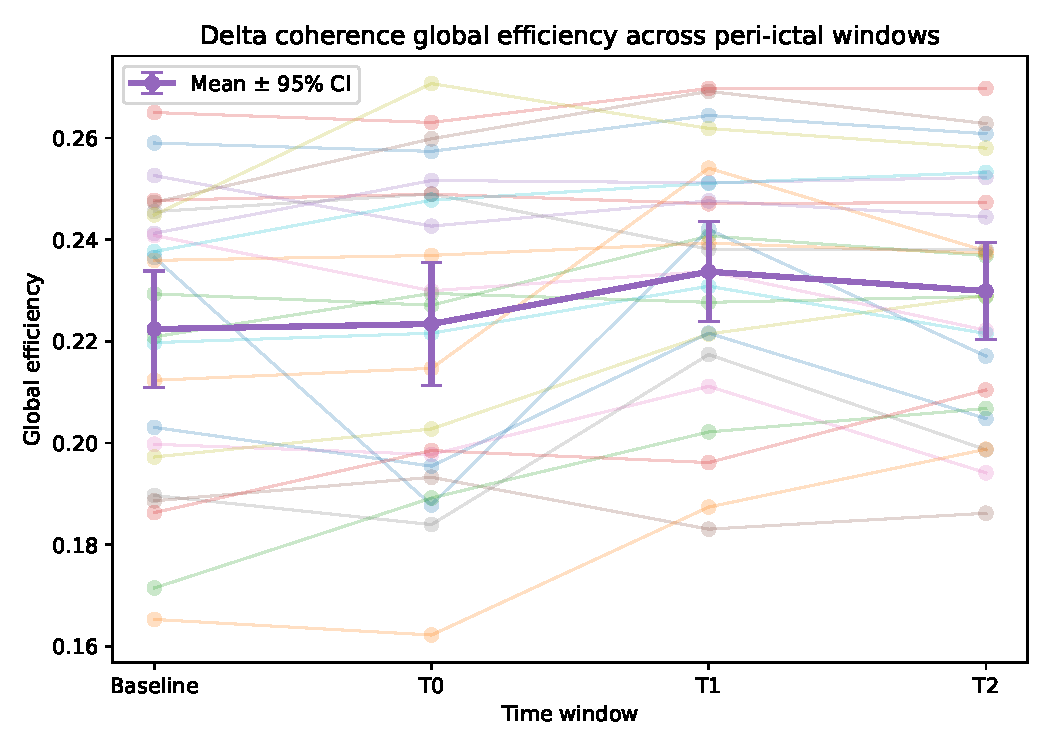
\includegraphics[width=0.85\textwidth]{figures/global_efficiency_coherence_delta_subject_average.pdf}
    \caption{Subject-average trajectory of delta-band coherence global
    efficiency across Baseline, T0, T1, and T2. Each subject/case identifier
    contributes one averaged value per temporal window.}
    \label{fig:global-efficiency-coherence-delta-subject-average}
\end{figure}

As shown in \cref{fig:global-efficiency-coherence-delta-subject-average}, the
subject-average trajectory increased from Baseline toward the preictal windows,
with the highest mean value in T1. This supports the seizure-level omnibus
finding by showing that the same pattern was present after averaging across
seizures within each subject/case identifier.

However, none of the subject-average Baseline-vs-preictal post-hoc contrasts
survived FDR correction. The Baseline-vs-T1 contrast showed the strongest
uncorrected effect
($t(23) = 4.40$, $p_{\mathrm{uncorrected}} = 0.000206$,
$p_{\mathrm{FDR}} = 0.089102$, Cohen's $d_z = 0.899$), but it did not meet the
corrected significance threshold. Therefore, the subject-average analysis
confirmed the overall temporal-window effect but did not localize a specific
Baseline-vs-preictal contrast after correction.

No other subject-average omnibus test survived FDR correction. Thus, the
subject-average analysis supported the main result observed at the seizure
level: delta-band coherence global efficiency was the only graph feature that
showed a robust temporal-window effect across both analysis levels.

\section{Summary of Main Findings}
\label{sec:results-summary-main-findings}

The full-dataset statistical analysis identified one robust graph-theoretical
effect after FDR correction. Global efficiency computed from delta-band
coherence networks showed a significant temporal-window effect in both the
seizure-level and subject-average omnibus analyses.

At the seizure level, the effect was localized by the planned post-hoc
comparisons to an increase from Baseline to T1. Mean global efficiency increased
from \num{0.224424} at Baseline to \num{0.233575} at T1, and this contrast
remained significant after FDR correction. The Baseline-vs-T2 comparison showed
the same direction of change but did not survive correction.

The preictal trend analysis did not identify any FDR-significant monotonic
T0--T1--T2 changes. Therefore, the main result should not be interpreted as a
strict linear increase toward seizure onset. Instead, the strongest evidence was
for a window-specific increase in delta-band coherence global efficiency,
especially around the T1 interval.

The subject-average sensitivity analysis supported the main finding at the
level of subject/case identifiers. The same metric--method--band combination
showed a significant omnibus window effect after averaging seizures within each
subject/case identifier. However, subject-average post-hoc contrasts did not
survive FDR correction, indicating that the localized Baseline-vs-T1 effect was
stronger at the seizure level than at the subject-average level.

No other graph metric, connectivity method, or frequency band combination
survived FDR correction in the omnibus, post-hoc, or trend analyses. Overall,
the results suggest that the most consistent preictal network alteration in this
dataset was a change in global integration of delta-band coherence networks,
rather than a broad effect across all graph metrics or all frequency bands.

    % \chapter{Discussion}

This chapter will interpret the findings in relation to seizure prediction, functional brain networks, and prior literature.

Limitations such as single-subject validation, small number of seizures, thresholding choices, and sensitivity to connectivity estimation will be discussed.



    % \chapter{Conclusions and Future Work}

This chapter will summarize the thesis contributions and outline future work.

Future directions may include multi-subject validation, predictive modeling, robustness analysis across graph thresholds, and improved clinical interpretability.



    % ----------------------------------------------------------------------
    % Appendices
    % ----------------------------------------------------------------------

    \appendix

    \chapter{Reproducibility}

This appendix will document the computational environment, repository structure, pipeline scripts, parameter choices, and data-management decisions used in the thesis.

Raw EEG data, processed arrays, connectivity matrices, graph metrics, and large generated outputs are intentionally excluded from this writing repository.



    % ----------------------------------------------------------------------
    % Bibliography
    % ----------------------------------------------------------------------

    \printbibliography[heading=bibintoc]

    % ----------------------------------------------------------------------
    % Acknowledgements
    % ----------------------------------------------------------------------

    \acknowledgements

    I would like to thank my supervisors for their guidance and support
    throughout this thesis. I am also grateful to my family, friends, and
    colleagues for their encouragement during the development of this work.

\end{document}